\documentclass{SEDESOLab}
\usepackage{ifthen}
% \usepackage[printonlyused,nohyperlinks]{acronym}
\usepackage{acronym}
\usepackage{units}

\usepackage{todonotes}
\usepackage[utf8]{inputenc}
\usepackage{siunitx}
\usepackage{subcaption}
\usepackage{hyperref}

\usepackage{csquotes}
\usepackage{dirtytalk}
\usepackage{supertabular}
\usepackage[section]{placeins}

\newcommand{\img}{./img}
\newcommand{\bib}{./bib}

\newcommand{\e}[1]{\mbox{e}^{#1}}
\graphicspath{{figures/}}



\begin{document}

%% Enter the deliverable information  in this document (tittle.tex)

%%%%%%%%%%%%%%%%%%%%%%%%%%%%%%%%%%%%%%%%%%%%%%%%%%%%%%%%%%%%%%%%%%%%%%%%%%%%%%%%%%
% First Page
%%%%%%%%%%%%%%%%%%%%%%%%%%%%%%%%%%%%%%%%%%%%%%%%%%%%%%%%%%%%%%%%%%%%%%%%%%%%%%%%%%
\graphicspath{{images/}}

\newcommand{\MyName}{Mónica Zamudio López}
\newcommand{\Institution}{Laboratorio de Datos, SEDESOL}
\newcommand{\DelTitle}{Recolección y limpieza de información}
\newcommand{\DelNumber}{1}
\newcommand{\DelVersion}{0.1/1.0}
\newcommand{\Contrato}{ATN/OC 15822-RG}
\newcommand{\footertext}{\raisebox{3mm}{Entregable \DelNumber}}
\setlength{\footheight}{36pt}
\newcommand{\footerlogo}{\raisebox{3mm}{\leavevmode
\includegraphics[width=2cm]{bid}}}
\clearscrheadfoot
\pagestyle{empty}


% \begin{tikzpicture}[overlay,remember picture]
%   \draw [line width=1pt]
%   ($ (current page.north west) + (1cm,-1cm) $)
%   rectangle
%   ($ (current page.south east) + (-1cm,1cm) $);
% \end{tikzpicture}

\definecolor{SINetblue}{HTML}{07505B}
\newcolumntype{C}{ >{\centering\arraybackslash} m{4cm} }

\begin{center}
SEDESOL 2018
\vspace{0.1cm}

  \begin{center}


  % H2020 has no logo and no visual identity

  % 
\includegraphics[width=0.7\textwidth]{images/LOGO_FJR}
      \Large \MyName \\\vspace{5mm}
\begin{multicols}{2}

\includegraphics[width=0.35\textwidth]{images/bid}

\includegraphics[width=0.25\textwidth]{images/LOGO_FJR}
\end{multicols}
\begin{multicols}{2}

\includegraphics[width=0.4\textwidth]{images/sedesol}

\includegraphics[width=0.2\textwidth]{images/presidencia}
\end{multicols}


  \vspace{2mm}

  \end{center}
  \vspace{0.3cm}
  {\Large Título del proyecto: USO DE DATOS MASIVOS PARA LA EFICIENCIA DEL ESTADO Y LA INTEGRACIÓN REGIONAL\\}
    {\large Clave: \Contrato}\\
  \vspace{0.5cm}
  \Large Puesto: Científico de Datos Junior\\
  \vspace{1.0cm}

  \begin{spacing}{2.5}
    \textbf{\Huge \DelTitle}\\\vspace{10mm}
    \textbf{\Large Entregable número: \DelNumber} \\\vspace{10mm}
  \end{spacing}

  % \vspace*{\fill}

  %just to avoid warning :)
  \newcommand\undefcolumntype[1]{\expandafter\let\csname NC@find@#1\endcsname\relax}
  \newcommand\forcenewcolumntype[1]{\undefcolumntype{#1}\newcolumntype{#1}}
  \forcenewcolumntype{C}{ >{\arraybackslash} m{3cm} }


  % \begin{tabular}{C@{\hspace*{0cm}}l}
  %   % \includegraphics[scale=0.2]{images/logos/EU_Flag_320_213} &
  %   % \begin{tabular}{l}
  %   % {Funded by the European Union’s Horizon 2020 research and innovation programme}\\
  %   % {under the Marie Sklodowska-Curie Grant Agreement No. 699924}\\
  %   \end{tabular}
  % \end{tabular}
\end{center}

\clearpage

%%%%%%%%%%%%%%%%%%%%%%%%%%%%%%%%%%%%%%%%%%%%%%%%%%%%%%%%%%%%%%%%%%%%%%%%%%%%%%%%%%
% Second Page
%%%%%%%%%%%%%%%%%%%%%%%%%%%%%%%%%%%%%%%%%%%%%%%%%%%%%%%%%%%%%%%%%%%%%%%%%%%%%%%%%%
\setlength{\headheight}{0.7cm}
\setlength{\footskip}{18mm}
\addtolength{\textheight}{-\footskip}
\pagestyle{empty}

\begin{flushright}
    \begin{tabular}{lp{11cm}}
    \textbf{Acrónimo del proyecto:}       &   Estimación de Ingreso \\
    \hline
    \textbf{Nombre completo del proyecto:} & USO DE DATOS MASIVOS PARA LA EFICIENCIA DEL ESTADO Y LA INTEGRACIÓN REGIONAL\\
    \hline
    \textbf{Referencia:}                  &   ATN/OC 15822-RG\\
    \hline
%    \textbf{Topic:}                 &   ICT-10-2015 \\
%    \textbf{Type of Action:}        &   RIA \\
    % \textbf{Grant Number:}          &   699924 \\
    \textbf{URL del Proyecto:}           &  \url{http://www.plataformapreventiva.gob.mx}
  \end{tabular}



% define "struts", as suggested by Claudio Beccari in
%    a piece in TeX and TUG News, Vol. 2, 1993.
\newcommand\Tstrut{\rule{0pt}{2.6ex}}         % = `top' strut
\newcommand\Bstrut{\rule[-0.9ex]{0pt}{0pt}}   % = `bottom' strut

  \begin{tabular}{|l|p{115mm}|}\hline
    % \Tstrut\Bstrut Editor:& XXX, XXX-Institution\\\hline
    \Tstrut\Bstrut Tipo de Entregable:& Reporte (R) \\\hline
    % \Tstrut\Bstrut Dissemination level:& Public (PU)\\\hline
    \Tstrut\Bstrut Fecha de Entrega Contractual:& Mayo - 2018\\\hline
    \Tstrut\Bstrut Fecha de Entrega& 3 de Mayo de 2018\\\hline
    % \Tstrut\Bstrut Suggested Readers:&Project partners, future community-lab.net users\\\hline
    \Tstrut\Bstrut Número de Páginas:&\pageref{finalpg}\\\hline
    \Tstrut\Bstrut Keywords:& estimación ingreso ciencia datos ingesta \\\hline
    \Tstrut Autor:&
    \begin{tabular}[t]{l}
      \MyName, \Institution \Bstrut \\
      % XXX - YYY, Institution \\
      % XXX - YYY, Institution \\
      % XXX - YYY, Institution \Bstrut \\
    \end{tabular}\\\hline
  \end{tabular}
\end{flushright}

\section*{Resumen}
La Secretaría de Desarrollo Social (SEDESOL) es una entidad del gobierno mexicano destinada al apoyo de la población para el mejoramiento de sus condiciones de vida.\\
Un problema importante para SEDESOL es la correcta distribución de sus recursos por lo que es importante contar con una metodología que permita la generación de una focalización correcta para así poder ayudar a aquellos que realmente están en condiciones vulnerables.\\
En este reporte se detalla el proceso de obtención e integración de distintas fuentes de información que puedes ser de utilidad en dicho proceso, ya sea de manera directa o como auxiliar de las primeras.\\
Las partes fundamentales para la realización de esto son, el estudio y evaluación de información generada por la misma Secretaría como lo es el Cuestionario Único de Información Socioeconómica (CUIS) y el Sistema de Focalización de Desarrollo (SIFODE), además de datos auxiliares que permitan la georreferenciación como archivos poligonales de carreteras y caminos. Para esto es importante llevar a cabo un sistema semiautomatizado para almacenar de manera adecuada todas las fuentes de datos para su futuro uso así como la información de los orígenes y naturaleza de las mismas.
\clearpage






% \oddsidemargin=5mm
% \evensidemargin=5mm
% \textwidth=30cm

% \topmargin=0cm
% \textheight=40\baselineskip
\setcounter{tocdepth}{2}

\tableofcontents
\listoffigures
\begingroup
\let\clearpage\relax
\listoftables
\endgroup

%% SHOULD be included if the deliverable becomes large
% \input{executivesummary}

%% COMMANDS
%%
%% \acresetall	flushes the ’memory’ of the macro \ac (ie all "used" marks flushed)
%%
%% \ac{label}	singular (first time Full Name + (ACRO) and mark as used)
%% \acp{label}	plural (as \ac but makes short and/or long forms into plurals)
%%
%% \acs{lable}	short (ACRO)
%% \acf{lable}	“full acronym” (Full Name + (ACRO))
%% \acl{lable}	long (_without_ ACRO)
%%
%% \acsp{label}	short plural (ACROs)
%% \acfp{label}	“full acronym” plural (Full Names + (ACROs))
%% \aclp{label}	long plural (_without_ ACRO)
%%
%% \acrodef{label}[acronym]{written out form}	definition
%%		for example \acrodef{etacar}[$\eta$ Car]{Eta Carinae},
%%		with the restriction that the label should be simple ASCII


%% PACKAGE & OPTIONS
%% acronym package must be loaded (in the preamble):
%%    \usepackage[option1,option2,etc.]{acronym}
%% OPTIONS:
%%    footnote		The option footnote makes the full name appear as a
%%			footnote.
%%    nohyperlinks	If hyperref is loaded, all acronyms will link to their
%%			glossary entry. With the option nohyperlinks these
%%			linkscan be suppressed.
%%    printonlyused	Only list used acronyms
%%    withpage		In printonlyused-mode show the page number where
%%			each acronym was first used.
%%    smaller		Make the acronym appear smaller.
%%    dua			The option dua stands for “don’t use acronyms”. It
%%			leads to a redefinition of \ac and \acp, making the
%%			full name appear all the time and suppressing all
%%			acronyms but the explicity requested by \acf or \acfp.
%%    nolist		The option nolist stands for “don’t write the list of
%%			acronyms”.


%% INCLUSION
%%
\chapter*{Lista de Acrónimos}
\label{sec:acronimos}

\begin{acronym}[ENIGH] %width of the longest acronym should be matched here
    \acro{DGGPB}{Dirección General de Geoestadística y Padrones de Beneficiarios}
    \acro{DGAE}{Dirección General Adjunta de Análisis Espacial}
    \acro{DGAIP}{Dirección General Adjunta de Integración de Padrones}
  \acro{CUIS}{Cuestionario Único de Información Socioeconómica}
  \acro{SIFODE}{Sistema de Focalización de Desarrollo}
  \acro{SEDESOL}{Secretaría de Desarrollo Social}
  \acro{ENIGH}{Encuesta Nacional de Ingresos y Gastos de los Hogares}
  \acro{PEA}{Población Económicamente Activa}
  \acro{LGDS}{Ley General de Desarrollo Social}
  \acro{INEGI}{Instituto Nacional de Estadística y Geografía}
  \acro{SISI}{Sistema de Información Social Integral}
  \acro{PUB}{Padrón Universal de Beneficiarios}
  \acro{AWS}{Amazon Web Services}

\end{acronym}
\clearpage


% ------------------------
% Chapter
% ------------------------

\clearscrheadfoot

% uncomment for book mode
%\lofoot{\footerlogo}
%\refoot{\footerlogo}
%\lefoot{\footertext}
%\rofoot{\footertext}

%\rohead{\pagemark}
%\lohead{\DelTitle}
%\lehead{\pagemark}
%\rehead{\DelTitle}

%\cfoot[\pagemark]{}

\lofoot[\footerlogo \hspace{10pt} \footertext]{\footerlogo \hspace{10pt} \footertext}
\lefoot[\footerlogo \hspace{10pt} \footertext]{\footerlogo \hspace{10pt} \footertext}

\refoot[\pagemark]{\pagemark}
\rofoot[\pagemark]{\pagemark}

\rohead{\rightmark}
\rehead{\rightmark}

\lohead{\leftmark}
\lehead{\leftmark}




\setcounter{page}{1}
\pagestyle{scrheadings}

\chapter{Introducción}
\section{Sección Uno}

\section{Sección Dos}

\chapter{Fuentes de datos}
\label{chap:fuentes}
\section*{Fuentes principales}
Para una tarea como la de identificar la falsa representación del estatus socioeconómico de los usuarios -activos y potenciales- de los distintos programas, es primordial contar con toda la información socioeconómica reportada que sea posible, e integrarla con la información disponible sobre las estrategias de focalización de los programas. En SEDESOL, la mayor parte de esta información es integrada por la DGAE y DGAIP, y compartida con el Laboratorio de Datos a través de nuestros recursos de almacenamiento en AWS\footnote{En particular, utilizamos el servicio S3 (Simple Storage Service) de Amazon Web Services. Esto es explicado con más detalle en el \autoref{chap:ingesta}}, salvo las excepciones que precisaremos conforme sea necesario.
\subsection*{CUAPS}
El \textbf{Cuestionario} \textbf{Único} \textbf{de} \textbf{Aplicación} \textbf{a} \textbf{Programas} es una herramienta utilizada por SEDESOL para obtener información de diseño y focalización de  los programas sociales. Para la integración de los datos, la DGAE envía anualmente un formato en Excel a los responsables de programas. A partir de 2017, se ha buscado migrar gradualmente a un llenado a través de la plataforma de SISI, por lo que la DGAE integra manualmente ambas fuentes de datos, y los envía al equipo del Laboratorio de Datos en formato \textit{.xlsx} Los datos de CUAPS son entregados al laboratorio en tres tablas distintas:
\begin{itemize}
    \item \textbf{Programas} - Esta tabla contiene los datos de diseño a nivel programa. Se especifica información administrativa del programa, sus objetivos generales y específicos de diseño, y los derechos sociales que el programa busca atender.
    \item \textbf{Componentes} - Para operar la política social, los programas definen apoyos que responden a los objetivos definidos en su diseño. Estos apoyos son la unidad más granular de suministro de beneficios utilizada por los programas, y pueden estar clasificados dentro de “bloques temáticos” llamados componentes.\footnote{Como un ejemplo simple: un programa de Mejoramiento a la Vivienda puede tener componentes de pisos, muros y techos, y otorgar tres apoyos diferentes para la componente de muros: cemento, varillas y un subsidio al salario de trabajadores de la construcción.}
    \item \textbf{Focalización} - Esta tabla contiene información de la focalización de programas, a nivel criterio de focalización. Los programas pueden tener uno o más criterios de focalización para definir a su población objetivo, y estos criterios pueden estar lógicamente relacionados. A partir de la información de la tabla, es posible reconstruir esas matrices de diseño y delimitar la población objetivo de los apoyos otorgados por los programas.
\end{itemize}
Dadas las diferencias entre las unidades observacionales, los datos son ingresados a nuestro catálogo como tres tablas distintas.
\subsection*{PUB}
El \textbf{Padrón Único de Beneficiarios} es el resultado de la consolidación de todos los padrones de los distintos programas sociales, conformado con el fin de monitorear los apoyos que reciben los beneficiarios. La actualización de los padrones es trimestral, y potencialmente corrige observaciones de trimestres anteriores al trimestre de actualización. En el PUB se tiene el nombre, sexo y grupo de edad del beneficiario, e información básica del programa del cual es beneficiario. Los datos del PUB son enviados por la DGAIP al equipo del laboratorio periódicamente, en formato .txt
\subsection*{CUIS-ENCASEH}
El Cuestionario Único de Información Socioeconómica es el instrumento mínimo\footnote{Los programas pueden hacer más preguntas de las que se incluyen en el CUIS, pero no menos.} utilizado por los programas para hacer levantamientos socioeconómicos, y es aplicado a nivel hogar. El CUIS puede aplicarse para procesos de identificación, recertificación, evaluación y verificación de los hogares, entre otros. Cada programa gestiona los datos para su operación, y la información que corresponde al CUIS se va integrando a lo largo del tiempo por la DGAE. La DGAE recibe la información del CUIS de dos formas: en un flujo continuo, a través de aplicaciones móviles, y en \textit{batch}, por parte de programas que cuentan con su propia infraestructura, como PROSPERA y LICONSA. Así, la dirección cuenta con datos históricos de los hogares que alguna vez han sido sujetos a levantamientos socioeconómicos, y a su vez integra periódicamente bloques de actualizaciones del CUIS. Los datos históricos son compartidos con el laboratorio a través de S3, en formato \textit{.zip} , separando cada tabla en un archivo distinto, mientras que los bloques de actualizaciones forman parte de SIFODE. Las tablas que tenemos disponibles son:
\begin{itemize}
    \item \textbf{domicilios}: contiene información no granular de la ubicación de la vivienda: estado, municipio y localidad para cada clave de hogar.
    \item \textbf{encuesta}: contiene información principalmente administrativa sobre la aplicación del cuestionario como el tipo de procedimiento, datos de la creación del registro en el sistema y el origen del levantamiento del cuestionario\footnote{El cuestionario puede ser levantado en aplicaciones móviles, cuestionarios en papel u otras modalidades.}.
    \item \textbf{ids}: contiene columnas utilizadas para relacionar distintas tablas con información a nivel hogar y persona.
    \item \textbf{integrante}: contiene datos de cada persona como integrante del hogar, como su condición de residencia y su parentesco con el jefe del hogar.
    \item \textbf{persona}: contiene datos administrativos sobre cada integrante del hogar.
    \item \textbf{se\_integrante}: contiene información socioeconómica a nivel persona, de cada integrante del hogar. Esto incluye temas de educación, discapacidad y ocupación, entre otros.
    \item \textbf{se\_vivienda}: contiene información socioeconómica sobre el hogar en su conjunto, como las características de la vivienda, el acceso de sus integrantes a las instituciones de salud y los proyectos productivos que realizan los integrantes del hogar.
    \item \textbf{vivienda}: contiene información principalmente administrativa sobre la vivienda, como el tipo de vivienda y el total de personas en ella.
\end{itemize}
\par
\noindent
Existen muchos programas que hacen preguntas adicionales al CUIS en sus levantamientos. Un caso de especial interés para este proyecto es el de PROSPERA, tanto por su tamaño\footnote{PROSPERA representa alrededor de la mitad de los beneficiarios registrados en el PUB.} como por su dinámica: dentro de sus levantamientos, PROSPERA cuenta con un módulo adicional de verificaciones domiciliarias, que representa un insumo extremadamente importante para un proyecto como el nuestro. Más adelante se explica el contenido de este módulo con mayor detalle.
\subsection*{SIFODE}
El Sistema de Focalización de Desarrollo es una herramienta diseñada para coordinar la operación de los programas sociales, administrada dentro de la DGAE. En esencia, su operación consiste en utilizar la información socioeconómica de los hogares con los que se cuenta para crear universos potenciales de personas beneficiarias de los programas sociales. Para esta tarea, se toman bloques temporales de datos del CUIS y del PUB, y se genera información sobre la situación de ingreso y carencias sociales enfrentada por los hogares encuestados. Estos elementos son los factores que componen la definición de pobreza multidimensional\footnote{Ver \cite{coneval_folleto} para más detalle} del Consejo Nacional de Evaluación de la Política de Desarrollo Social (CONEVAL):
\begin{itemize}
    \item Ingreso corriente per cápita - el ingreso compone la detección de pobreza y vulnerabilidad a través de dos puntos de corte: la Línea de Bienestar Económico\footnote{Esta especifica el ingreso necesario para adquirir las canastas alimentaria y no alimentaria de bienes y servicios. Ver \cite{coneval_medicion} para mayor detalle.} y la Línea de Bienestar Mínimo.\footnote{Esta especifica el ingreso necesario para adquirir la canasta alimentaria.}
    \item Rezago educativo - El indicador de rezago educativo toma como elementos el acceso a la educación obligatoria correspondiente que tienen los distintos integrantes de los hogares. La persona se considera como no carente sólo si está en edad escolar y asiste a la escuela o si de acuerdo con su edad ha concluido la primaria o secundaria, considerando la legislación aplicable.
    \item Acceso a los servicios de salud - El indicador de acceso a los servicios de salud toma en consideración que las personas cuenten con adscripción o derecho a recibir servicios médicos en alguna institución de salud, ya sea pública o privada. La persona se considera como no carente sólo si cuenta con adscripción o filiación directa o indirectamente a alguna institución de este tipo.
    \item Acceso a la seguridad social - El indicador de acceso a la seguridad social toma en cuenta el acceso de las personas a coberturas sociales mínimas que deben otorgarse a los trabajadores y a sus familias. La seguridad social puede definirse como \textit{''el conjunto de mecanismos diseñados para garantizar los medios de subsistencia de los individuos y sus familias ante eventualidades como accidentes, enfermedades, la vejez o el embarazo.''}\footnote{Ver \cite{coneval_folleto}.}
    \item Calidad y espacios de la vivienda - El indicador de calidad y espacios en la vivienda toma en consideración que la vivienda cuente materiales que garanticen la estabilidad y firmeza de los pisos, techos y muros, así como que las personas que la habitan no vivan en condiciones de hacinamiento.
    \item Acceso a los servicios básicos en la vivienda - El indicador de acceso a los servicios básicos en la vivienda considera las condiciones sanitarias en las que viven las personas habitantes de la vivienda. En particular, se considera que dichas personas carecen de servicios básicos en la vivienda si la vivienda no cuenta con agua entubada dentro del terreno, drenaje y electricidad o si el combustible usado para cocinar es carbón, y la vivienda no cuenta con chimenea.
    \item Acceso a la alimentación - El indicador de acceso a la alimentación es construido a partir de la Escala Mexicana de Seguridad Alimentaria, y toma en consideración si las integrantes de la vivienda tuvieron alimentación basada en poca variedad, dejaron de tomar al menos una de las tres comidas del día, comieron menos de lo que piensan debían comer, se quedaron sin comida o sintieron hambre pero no comieron.
    \item Grado de cohesión social - El CONEVAL define tres espacios conceptuales para medir el desarrollo social de los mexicanos: el bienestar, los derechos sociales y el contexto territorial. El primero es medido a través de los cortes antes mencionados al ingreso, el segundo por los indicadores de acceso mencionados, y el último por el grado de cohesión social en el espacio del territorio. Las propuestas retomadas por CONEVAL con respecto a su conformación comprenden la desigualdad económica, la razón de ingreso entre la población en pobreza extrema y la no pobre y no vulnerable, la polarización social y las redes sociales. Sin embargo, no existe un consenso sobre los indicadores a utilizar, así que el grado de cohesión social constituye una dimensión teórica de la pobreza multidimensional pero no de su medición actualmente.
\end{itemize}
Una vez obtenidos esos indicadores de bienestar y carencias, esta información es integrada con los datos del PUB, para así generar universos de beneficiarios potenciales de programas y entonces optimizar la frecuencia de los levantamientos socieconómicos.
\par
\noindent
El SIFODE es integrado cada año por la DGAE, y compartido con el laboratorio a través de S3 en archivos \textit{rar} separados por tablas. Si bien se cuenta con la información histórica de los cuestionarios aplicados a todos los hogares, el sifode toma únicamente la última ''fotografía'' obtenida por el CUIS en cada hogar. Así, contamos tanto con tomas aisladas de CUIS e integradas a SIFODE, como con la información histórica de los hogares. Esto nos permite reconstruir la trayectoria de ingreso y carencias que han vivido los hogares a través del tiempo.
\subsection*{Módulo de verificaciones}
Como se especificó anteriormente, PROSPERA es uno de los programas que tiene un cuestionario más completo que el CUIS. Uno de sus componentes más importantes es el módulo de verificaciones domiciliarias. Eso es especialmente relevante, porque no todos los cuestionarios son aplicados en el domicilio de las personas, y aún de serlo las personas pueden tener oportunidad de mentir en más de un aspecto de las características de su vivienda o su estilo de vida. La posibilidad de comparar entre datos reportados y datos verificados nos permite generar modelos considerando variables faltantes o latentes. Dado que PROSPERA es independiente de la DGGPB, los datos de sus cuestionarios y módulos de verificacion son compartidos con el laboratorio a través de un convenio de colaboración, en el que el laboratorio obtuvo los datos de verificaciones y cuestionarios anuales entre los años 2010 y 2017. Se tienen tablas separadas por tipo de visita (verificaciones u otro tipo de aplicación del cuestionario) y por año, en formato \textit{DBF.}
\section*{Fuentes adicionales}
Para complementar los modelos de ingreso, existen otras fuentes de datos que pueden explotar la relación espacial que guardan las distintas aplicaciones de cuestionarios, como lo son la red carretera de INEGI, los datos georeferenciados de INEGI y el PUB georeferenciado. Estas fuentes de datos generalmente provienen de servicios web que permiten descargar archivos comprimidos de tipo \textit{ZIP, RAR, TAR}, etc., y contienen \textit{shapefiles} con los polígonos que integran el mapa. Estos archivos son convertidos a formato \textit{CSV} para su posterior ingesta.

\chapter{El proceso de ingesta}
\label{chap:ingesta}
\section*{Infraestructura}
Como ya hemos explicado, la naturaleza del proyecto implica obtener, procesar, transformar e integrar múltiples fuentes de datos. Con eso en mente, hemos ensamblado una infraestructura orientada a fuentes de datos. Esa infraestructura responde a varias necesidades:
\begin{itemize}
    \item \textbf{Escalabilidad} - las exigencias de memoria y procesamiento de nuestros flujos de extracción, transformación y carga (comúnmente llamados ETL, por sus siglas en inglés) pueden variar considerablemente con el tamaño de las bases de datos. Así, para datos como los padrones o cuestionarios largos sería óptimo correr 10 procesos en paralelo, mientras que para cuestionarios pequeños como CUAPS esa capacidad sería mal aprovechada.
    \item Portabilidad - es también importante que ningún proceso quede supeditado a ser ejecutado en una plataforma o sistema operativo en particular, para así disminuir las necesidades de mantenimiento del código.
    \item \textbf{Seguridad} - dado el tipo de información con el que contamos, debemos garantizar la seguridad y privacidad de los datos sin comprometer la flexibilidad de agregar nuevos colaboradores al proyecto de ser necesario.
    \item \textbf{Actualización periódica y eficiente} - al tener un flujo continuo de datos hacia nuestros modelos, necesitamos que esos procesos ETL puedan ser replicados sin mayor esfuerzo. Asimismo, queremos evitar que alguna tarea sea repetida innecesariamente.
    \item \textbf{Documentación} - para que pueda ser replicado con facilidad, es necesario que cualquier persona con acceso al código pueda entender el flujo de datos, la serie de procesos que deben ocurrir y las fuentes de datos necesarias para replicar el análisis.
\end{itemize}
Considerando estas necesidades, usamos varias partes móviles para el proceso de ETL. Todos nuestros procesos son ejecutados en un servidor de AWS EC2, que tiene montado un disco EBS para almacenamiento del código. En ese servidor se construye un contenedor de Docker a partir de una imagen privada con sistema operativo Linux Debian, que cuenta con Python, R y los paquetes necesarios para ejecutar el proyecto. La mayor parte de nuestras necesidades de almacenamiento de datos a través del flujo ETL se llevan a cabo en AWS S3, para al final escribirse a una base de datos AWS RDS en PostgreSQL. Por último, tenemos un registro del linaje de los datos en una base de datos orientada a grafos, en Neo4j.
\par
\noindent
Para facilitar la actualización periódica de los datos, todo el flujo está orquestado en Luigi con las tareas como sigue:
\par
\noindent
\begin{figure}[h]
    \caption{Flujo de datos}
    \centering
    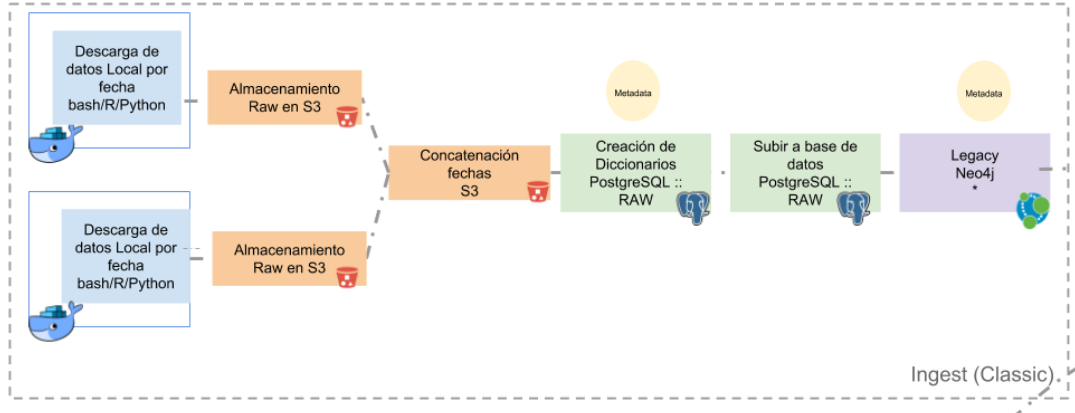
\includegraphics[width=\textwidth]{ingest_pipeline.png}
\end{figure}
Así, todas nuestras fuentes de datos son ingestadas concatenando el conjunto de datos históricos antes de escribirse a la base de datos. Cada fuente de datos tiene su propio script de ingesta local, escrito ya sea en \textit{bash, python} o \textit{R} que toma como parámetros la fecha del dato, el nombre de la fuente y la ruta de descarga local al servidor.
\par
\noindent
Para tener un registro ordenado de la metadata, utilizamos el estándar DCAT
\section*{Scripts de ingesta}
Para ingestar los archivos de CUIS, es necesario utilizar los paquetes \textit{unzip} y \textit{unrar}\cite{unrar_debian, unzip_debian}, que permiten la descompresión de archivos, y \textit{csvkit} \cite{csvkit}, un paquete de \textit{python} con integración a \textit{bash} que permite aplicar distintas transformaciones a datos de tipo CSV, incluyendo la conversión a CSV desde archivos de Excel.
Todos los códigos de ingesta están disponibles en el \autoref{chap:apendice}.


\chapter{Conclusiones}

Lorem ipsum dolor sit amet, consectetur adipiscing elit. Pellentesque rutrum nec dui nec dignissim. Pellentesque eget augue luctus nisl mollis malesuada. Vestibulum ultricies dapibus magna, vitae suscipit est condimentum sed. Vivamus sed sem ut mauris placerat aliquet nec quis ligula. Donec ac tortor erat. Duis ac augue sed urna laoreet finibus ac eu erat. Fusce placerat blandit arcu, ut mattis turpis luctus eu. Phasellus eleifend orci vulputate pharetra rhoncus. Nulla vitae interdum purus, vel posuere arcu. Donec at faucibus purus. Nam sodales tincidunt arcu ut vestibulum. Aliquam enim mi, tempor ac placerat in, gravida vitae augue. Donec lacinia accumsan justo non tincidunt. Curabitur porttitor quam in scelerisque tempus. Ut maximus elementum massa et egestas.

Ut interdum orci sed faucibus elementum. Maecenas vulputate metus non nulla finibus rutrum. Nullam eleifend ex id metus euismod, vel consectetur ex elementum. Sed efficitur libero non diam fermentum vehicula. Nunc dignissim suscipit libero, a feugiat nunc lacinia vitae. Sed at mollis nibh, mattis tincidunt dolor. Suspendisse maximus mi metus, vulputate hendrerit justo volutpat nec. Etiam vitae dui iaculis, pulvinar ante eu, congue leo. Fusce efficitur nunc massa, vel tincidunt velit accumsan in.

Vestibulum at nulla nunc. Sed sed lorem orci. Mauris ut porta diam. Quisque ac euismod quam. Phasellus tempor tempor tellus. Sed bibendum turpis at vehicula vulputate. Quisque condimentum efficitur lectus, vitae vehicula enim dapibus accumsan. Nullam bibendum, orci non scelerisque gravida, metus sapien pulvinar turpis, pulvinar egestas tellus sapien ut sem.

Nullam consequat elit quis ipsum imperdiet, ac placerat leo cursus. Proin cursus sit amet urna ut rutrum. Fusce congue elit non elit iaculis fermentum. Nullam quis ex nec dolor lobortis porta. Quisque enim lorem, pretium nec velit ut, eleifend laoreet magna. Vivamus eu mauris at purus sagittis condimentum. Nunc congue accumsan mauris, at convallis lacus pharetra in. Cras bibendum orci urna, nec elementum ex ornare sollicitudin. Praesent non ultricies velit. Curabitur volutpat malesuada enim, vel maximus libero vestibulum vitae. Curabitur rhoncus erat nibh, quis viverra orci euismod nec. Donec magna lacus, tempor vitae justo sed, vulputate pretium massa. Aenean diam est, eleifend sit amet pellentesque vel, fermentum iaculis tellus. Etiam dignissim congue tellus, eget eleifend ipsum sagittis ut. Fusce convallis sapien dui.

Vivamus pretium mauris quis ligula vestibulum hendrerit. Ut maximus, erat vitae congue faucibus, eros nunc fermentum erat, id ultricies felis erat ac neque. Maecenas risus nunc, aliquam et leo quis, venenatis hendrerit nisl. Nunc viverra elementum ex, eu efficitur quam mollis nec. Mauris odio enim, fermentum non nibh eu, vestibulum venenatis felis. Lorem ipsum dolor sit amet, consectetur adipiscing elit. Cras ac velit varius, congue eros non, fringilla sapien. Fusce pretium porttitor urna a accumsan. Duis pharetra lorem vel mauris vehicula, non accumsan lectus mattis. Suspendisse posuere massa eget velit venenatis, eget gravida turpis vulputate. Cum sociis natoque penatibus et magnis dis parturient montes, nascetur ridiculus mus. Duis convallis accumsan urna, convallis facilisis ipsum feugiat id. Nunc gravida, magna eu euismod pharetra, nulla risus porta urna, a dapibus augue lorem blandit justo.



\bibliography{bib/references}
\appendix
\chapter{Apéndice}
\lstinputlisting[language=bash,basicstyle=\ttfamily\scriptsize,caption={Archivo de ingesta de Red Carretera}]{code/red_carretera.sh}
\pagebreak
\lstinputlisting[language=bash,basicstyle=\ttfamily\scriptsize,caption={Archivo de ingesta de Sifode Calificación}]{code/sifode_calificacion.sh}
\pagebreak
\lstinputlisting[language=bash,basicstyle=\ttfamily\scriptsize,caption={Archivo de ingesta de Sifode Domicilio}]{code/sifode_domicilio.sh}
\pagebreak
\lstinputlisting[language=python,basicstyle=\ttfamily\scriptsize,caption={Archivo de ingesta de Sifode}]{code/sifode.py}
\pagebreak
\lstinputlisting[language=json,basicstyle=\ttfamily\scriptsize,caption={Catálogo},breaklines=true]{code/catalog.json}

\label{finalpg}
\clearpage

\thispagestyle{empty}
\begin{center}
% \vfill
% \begin{figure}
% \centering
% \vspace{3cm}
  % 
\includegraphics[width=10cm]{images/LOGO_FJR}

\begin{multicols}{2}

\includegraphics[width=0.35\textwidth]{images/bid}

\includegraphics[width=0.25\textwidth]{images/LOGO_FJR}
\end{multicols}
\begin{multicols}{2}

\includegraphics[width=0.4\textwidth]{images/sedesol}

\includegraphics[width=0.2\textwidth]{images/presidencia}
\end{multicols}

% \end{figure}
% \vfill
{\large USO DE DATOS MASIVOS PARA LA EFICIENCIA DEL ESTADO Y LA INTEGRACIÓN REGIONAL\\[0.5cm] }
{\large \today \\[0.5cm] }
{\large FJR-\DelNumber-\Contrato\\[0.5cm] }
\vfill

SEDESOL 2018

\doclicenseLicense
\end{center}


%\printbibliography
\end{document}
